\chapter{Il livello di rete}
\label{cap:livelloRete}
\thispagestyle{chapterInit}
\section{Visione d'insieme}
    \paragraph{Obbiettivo del livello di rete} L'obbiettivo principale del livello di rete è quello di permettere la comunicazione tramite reti diverse attraverso apparecchi detti \textit{router} i quali hanno il compito di inoltrare le informazioni verso la destinazione.
    \paragraph{Funzioni principali} Esistono due funzioni principali del livello di rete: \begin{description}
        \item[Inoltro \textit{forwarding}] Questa è una operazione a livello locale che consiste nel prendere un pacchetto in ingresso e inoltrarlo verso l'uscita corretta.
        \item[Instradamento \textit{routing}] Questa è una operazione a livello globale che consiste nel determinare il percorso migliore per inoltrare un pacchetto verso la destinazione. Per questa operazione si utilizzano degli algoritmi di \textit{routing}.
    \end{description}
    Queste due funzioni sono legate tra loro, ma possono essere isolate. Infatti convenzionalmente distinguiamo con \textit{control plane} la parte del livello di rete che si occupa dell'istradamento e con \textit{data plane} la parte che si occupa dell'inoltro. Questa distinzione è utile per capire come funzionano i router.
    \subparagraph{\textit{Data Pane}} Il \textit{data plane} ha funzione a livello locale ad ogni \textit{router}, questo è il livello che determina \underline{come} inoltrare un \textit{datagram} fornendo la funzione di \textit{forwarding}.
    \subparagraph{\textit{Control Plane}} Il \textit{control plane} ha funzione a livello globale, questo è il livello che determina \underline{dove} inoltrare un \textit{datagram} fornendo la funzione di \textit{routing}.
\section{Come è fatto un router}
    Visto a livello "alto" un router è composto da tre livelli principali: \begin{description}
        \item[Terminazione di linea] Questo è il livello più basso del router, è composto da un'interfaccia di rete che si occupa di ricevere i pacchetti e di inviarli al livello successivo.
        \item[Protocollo di livello \textit{data link}] Questo livello si occupa di ricevere i pacchetti dal livello precedente e di inviarli al livello successivo. Inoltre si occupa di fare il controllo degli errori e di gestire il flusso.
        \item[Inoltro e \textit{buffer}] Questo è il livello che si occupa di inoltrare i pacchetti verso la destinazione. Inoltre si occupa di fare il \textit{buffering} dei pacchetti in caso di congestione.
    \end{description}
    \subsection{Sistemi di commutazione}
        I sistemi di commutazione trasferiscono i pacchetti dalle porte di ingresso all'uscita appropriata. Definiamo come \textbf{tasso di comunicazione} la frequenza alla quale i pacchetti vengono portati dall'ingresso all'uscita (spesso è un multiplo della velocità di comunicazione) 
        \subsubsection{Commutazione a memoria}
            Questo è il metodo più semplice, i pacchetti vengono memorizzati in un buffer comune e poi inoltrati verso l'uscita appropriata. Questo metodo è molto semplice ma ha il problema che la velocità di inoltro è limitata dalla velocità di accesso alla memoria.
        \subsubsection{Commutazione a bus}
            Questo metodo consiste nel collegare le porte di ingresso e di uscita tramite un bus, sempre comune a tutte le porte. Questo metodo risulta lento in quanto non possono essere trasferiti più pacchetti contemporaneamente anche se le porte di ingresso e di uscita sono diverse. Il \texttt{Cisco 5600} è un esempio di router che utilizza questo metodo e riesce a trasferire fino a 32 Gbit/s.
        \subsubsection{Commutazione a matrice}
            Questo metodo consiste nel collegare le porte di ingresso e di uscita tramite una matrice di commutazione. Questo metodo è molto veloce in quanto permette di trasferire più pacchetti contemporaneamente in quanto se le porte sono differenti allora basta attivare i vari collegamenti della matrice. Questo metodo è molto veloce ed ispirato ai primi commutatori telefonici. Il \texttt{Cisco 12000} è un esempio di router che utilizza questo metodo e riesce a trasferire fino a 60 Gbit/s.
    \subsection{Accodamenti}
        Gli accodamenti sono utilizzati per evitare la perdita di pacchetti in caso di congestione dell'apparecchio di rete. Questo è un problema molto comune in quanto i router sono dispositivi molto veloci e le porte di uscita sono molto più lente. Per evitare la perdita di pacchetti si utilizzano delle code che permettono di memorizzare i pacchetti in attesa di essere inoltrati.
        Le code possono essere formate in ingresso, quando una stessa porta di uscita è condivisa da più porte di ingresso e quindi una porta di uscita può essere congestionata. Le code possono essere formate in uscita, quando una porta di uscita ha un \textit{link} più lento rispetto alla velocità di inoltro dei pacchetti tramite le porte di ingresso o il commutatore di pacchetto.
        \paragraph{Quanta memoria serve per i \textit{buffer}} Secondo \texttt{RFC 3439} la quantità di memoria necessaria per i buffer è data dalla formula: \[M = \frac{RTT \cdot C}{\sqrt{N}}\] Dove: \begin{description}
            \item[$M$] è la memoria necessaria per il buffer
            \item[$RTT$] è il tempo di round trip
            \item[$C$] è la capacità del collegamento
            \item[$N$] è il numero di connessioni
        \end{description}
        \paragraph{Meccanismi di \textit{scheduling}}
            I meccanismi di \textit{scheduling} sono utilizzati per decidere quale pacchetto inoltrare quando si ha la possibilità di inoltrare più pacchetti. Il meccanismo più semplice è il \textit{First In First Out} (\texttt{FIFO}) che inoltra i pacchetti in ordine di arrivo. Inoltre viene applicata una politica di scarto dei pacchetti in caso di buffer pieno. Questa politica può essere: \begin{description}
                \item[\textit{Drop Tail}] Questa politica scarta i pacchetti in arrivo quando il buffer è pieno.
                \item[\textit{Random Early Detection}] Questa politica scarta i pacchetti in arrivo in modo casuale quando il buffer è pieno.
                \item[\textit{Priority Drop}] Questa politica scarta i pacchetti in arrivo in base alla priorità.
            \end{description}
            La politica di scarto dei pacchetti dipende dall'implementazione del router.
\section{Il protocollo \texttt{IP}}
    \subsection{Il formato del \textit{datagram} \texttt{IP} (\texttt{IPv4})}
        \begin{figure}[H]
            \centering
            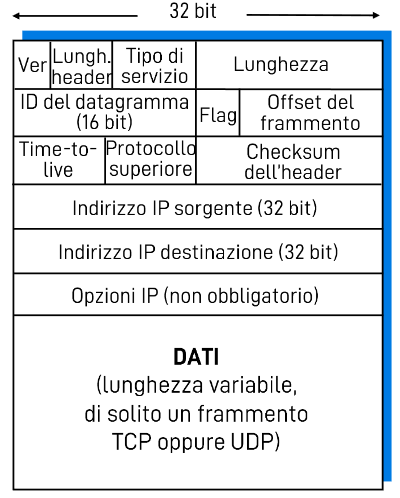
\includegraphics[width=0.36\textwidth]{04/datagramIPv4.png}
            \caption{Il formato del \textit{datagram} \texttt{IP} (\texttt{IPv4})}
            \label{fig:IPv4Header}
        \end{figure}
        Il formato del \textit{datagram} \texttt{IP} è composto da 20 byte di intestazione e da un campo dati. Il campo dati può contenere fino a 65.535 byte.  Di seguito si riportano i vari campi dell'intestazione:
        \begin{description}
            \item[VER] (4 bit) Questo campo contiene la versione del protocollo \texttt{IP} utilizzato.
            \item[Lunghezza \textit{header}] (4 bit) Questo campo contiene la lunghezza dell'intestazione in parole da 32 bit. (=5 se non ci sono opzioni)
            \item[Tipo di servizio - \texttt{ToS}] (8 bit) Questo campo contiene informazioni sul tipo di servizio richiesto.
            \item[Lunghezza totale] (16 bit) Questo campo contiene la lunghezza totale del \textit{datagram} in byte.
            \item[Identificativo] (16 bit) Questo campo contiene un numero univoco per il \textit{datagram}.
            \item[Flag] (3 bit) Questo campo contiene i flag per il frammento. Il primo bit è il bit di \textit{Don't Fragment}, il secondo bit è il bit di \textit{More Fragment} e il terzo bit è il bit di \textit{Fragment Offset}.
            \item[Offset] (13 bit) Questo campo contiene l'offset del frammento. (Espresso in multipli di 8 byte)
            \item[\textit{Time To Live} - \texttt{TTL}] (8 bit) Questo campo contiene il numero di \textit{hop} massimo che il \textit{datagram} può fare.
            \item[Protocollo] (8 bit) Questo campo contiene il protocollo di trasporto che si trova nel campo dati.
            \item[Checksum] (16 bit) Questo campo contiene il checksum dell'intestazione.
            \item[Indirizzo IP sorgente] (32 bit) Questo campo contiene l'indirizzo IP sorgente.
            \item[Indirizzo IP destinazione] (32 bit) Questo campo contiene l'indirizzo IP destinazione.
            \item[Opzioni] (variabile) Questo campo contiene le opzioni del \textit{datagram}.
            \item[Padding] (variabile) Questo campo contiene il padding per allineare l'intestazione a multipli di 32 bit.
        \end{description}
    \subsection{\texttt{MTU} e Frammentazione}
        La \texttt{MTU} (\textit{Maximum Transmission Unit}) è la dimensione massima di un pacchetto che può essere trasmesso su un collegamento, ogni \textit{hardware} specifica il proprio \texttt{MTU}. Se un \textit{datagram} è più grande della \texttt{MTU} allora il \textit{datagram} viene frammentato in pacchetti più piccoli. Questo processo è chiamato \textit{frammentazione}. I pacchetti frammentati vengono poi ricomposti alla destinazione.
        \paragraph{Valori Standard \texttt{MTU}} Per alcuni tipi di collegamenti sono stati definiti dei valori standard di \texttt{MTU}. Ad esempio per le reti Ethernet la \texttt{MTU} è di $1500$ byte, per le reti \texttt{WLAN 802.11} la \texttt{MTU} è di $2304$ byte,\dots. In un collegamento tra due \textit{host} possono essere presenti due valori di \texttt{MTU} diversi
        \subparagraph{Esempio} Supponendo che per raggiungere un host \texttt{B} si debba passare prima da una rete con $1500$ byte di \texttt{MTU} e poi da una rete con $1000$, tutto ciò tramite un router \texttt{R}. Allora quando il \textit{router} \texttt{R} riceve il datagram di $1500$ byte lo frammenta in due pacchetti di $1000$ byte e $500$ byte. I pacchetti vengono quindi inoltrati alla destinazione. Quando l'host \texttt{B} riceve i pacchetti li ricomponi e li passa al livello di trasporto.
        
    \subsection{Indirizzamento e \texttt{NAT}}
        \subsubsection{Indirizzi \texttt{IP}}
            Un indirizzo \texttt{IP} è composto da $32$ bit ed è associato ad un'interfaccia di rete. Una interfaccia è una connessione tramite mezzo fisico o logico, solitamente ogni \textit{host} ha una o più interfacce di rete.
            \paragraph{Caratteristiche indirizzi \texttt{IP}} Gli host e i router devono usare le stesse convenzioni per gli indirizzi \texttt{IP}, inoltre ogni indirizzo \texttt{IP} deve essere unico e raggiungibile da un qualsiasi punto di internet. Quando si invia un pacchetto \texttt{IP} si invia l'indirizzo \texttt{IP} sorgente e l'indirizzo \texttt{IP} destinazione. I \textit{router} sono apparati di rete che quando ricevono un pacchetto \texttt{IP} decidono dove inoltrarlo in base all'indirizzo \texttt{IP} di destinazione.
            \paragraph{Norazione indirizzo \texttt{IP}} Gli indirizzi \texttt{IP} sono composti da $4$ gruppi di $8$ bit e sono scritti in notazione decimale a punti. Ogni gruppo di $8$ bit è espresso in decimale e separato da un punto. Gli indirizzi disponibili vanno dà: $0.0.0.0$ a $255.255.255.255$ 
            \paragraph{Gerarchie indirizzi \texttt{IP}} Gli indirizzi \texttt{IP} sono organizzati in una struttura gerarchica. Inoltre solitamente sono divisi in due parti: \begin{description}
                \item[Parte di rete] Questa parte identifica la rete a cui appartiene l'indirizzo \texttt{IP}.
                \item[Parte di \textit{host}] Questa parte identifica l'\textit{host} all'interno della rete.
            \end{description}
            \subparagraph{Classi di indirizzi \texttt{IP}} Gli indirizzi \texttt{IP} sono divisi in classi sulla base dei primi bit dell'indirizzo e dalla lunghezza del prefisso: \begin{description}
                \item[Classe \texttt{A}] Gli indirizzi di classe \texttt{A} hanno il primo bit a \texttt{0} e sono composti da $8$ bit di rete e $24$ bit di \textit{host}. Gli indirizzi vanno da $0.0.0.0$ a $ 127.255.255.255$ e sono riservati per le reti molto grandi.
                \item[Classe \texttt{B}] Gli indirizzi di classe \texttt{B} hanno i primi due bit a \texttt{10} e sono composti da $16$ bit di rete e $16$ bit di \textit{host}. Gli indirizzi vanno da $128.0.0.0$ a $191.255.255.255$ e sono riservati per le reti di medie dimensioni.
                \item[Classe \texttt{C}] Gli indirizzi di classe \texttt{C} hanno i primi tre bit a \texttt{110} e sono composti da $24$ bit di rete e $8$ bit di \textit{host}. Gli indirizzi vanno da $192.0.0.0$ a $223.255.255.255$ e sono riservati per le reti di piccole dimensioni.
                \item[Classe \texttt{D}] Gli indirizzi di classe \texttt{D} hanno i primi quattro bit a \texttt{1110} e sono riservati per i \textit{multicast}.
                \item[Classe \texttt{E}] Gli indirizzi di classe \texttt{E} hanno i primi quattro bit a \texttt{1111} e sono riservati per usi futuri.
            \end{description}
        \subsubsection{Assegnazione indirizzi \texttt{IP}}
            Gli indirizzi \texttt{IP} sono assegnati dalla \texttt{ICANN} (\textit{Internet Corporation for Assigned Names and Numbers}) che riserva una intera classe ai \texttt{ISP} (\textit{Internet Service Provider}) e poi questi assegnano gli indirizzi ai propri clienti. Gli indirizzi \texttt{IP} sono assegnati in modo gerarchico e quindi un \texttt{ISP} può assegnare un intero blocco di indirizzi ad un altro \texttt{ISP} e questo può assegnare un blocco di indirizzi ad un altro \texttt{ISP} e così via.
    \subsection{Indirizzamento \textit{classless}}
        In quanto ci si è accorti che con la suddivisione degli indirizzi in classi si stava sprecando molti indirizzi, si è deciso di passare ad un indirizzamento \textit{classless}. Questo tipo di indirizzamento permette di avere una suddivisione più flessibile degli indirizzi, in quanto possiamo richiedere al nostro \texttt{ISP} solo un \textit{range} di indirizzi e non una classe intera, ad esempio l'\texttt{ISP} può usare un prefisso di $26$ bit per identificare la rete nel mondo e successivamente usare i restanti $6$ bit per identificare tutti gli \textit{host} della rete.
        In questa situazione se un \texttt{ISP} ha acquistato una rete di classe \texttt{C} e ha bisogno di dividere la rete in quattro clienti allora può dividere la rete in $4$ sotto-reti e assegnare un prefisso di $26$ bit ($24$ per la classe \texttt{C} e $2$ per le sotto-reti) e i restanti $6$ bit per gli \textit{host} di ogni sotto-rete.
        \subsubsection{Maschere di rete}
            In quanto ora non si ha più una suddivisione fissa degli indirizzi, si è deciso di introdurre le \textit{maschere di rete}. Queste maschere sono composte da $32$ bit e sono composte da una parte di $1$ quelli che identificano il prefisso di rete e da una parte di $0$ che identificano gli \textit{host} della rete. Ad esempio la maschera di rete per una rete di classe \texttt{C} è $11111111.11111111.11111111.00000000$.
            \paragraph{Peché si usa?} La maschera di rete viene usata per identificare la rete di appartenenza di un indirizzo IP. Per fare ciò si fa un'operazione di \texttt{AND} tra l'indirizzo IP di destinazione e la maschera di rete. Se il risultato è uguale all'indirizzo di rete allora l'indirizzo IP appartiene alla rete. Quindi se il prefisso di rete è $128.10.0.0$ ovvero: \[10000000.00001010.00000000.00000000\] e la maschera di rete è $255.255.0.0$ ovvero: \[11111111.11111111.00000000.00000000\] e l'indirizzo IP di destinazione di un determinato pacchetto è: $128.10.2.3$ ovvero: \[10000000.00001010.00000010.00000011\] allora facendo l'operazione di \texttt{AND} tra l'indirizzo IP e la maschera di rete si ottiene: \[\begin{aligned}
                10000000.00001010.00000010.00000011 &\\
                11111111.11111111.00000000.00000000 &\\
                \hline
                10000000.00001010.00000000.00000000&=128.10.0.0
            \end{aligned}
            \] Quindi l'indirizzo IP appartiene alla rete e il pacchetto viene inoltrato a quella determinata porta di uscita.
        \subsubsection{Notazioni \texttt{CIDR}}
            \texttt{CIDR} o \textit{Classless Inter-Domain Routing} è un metodo per rappresentare le maschere di rete. Questo metodo consiste nel rappresentare la maschera di rete con un prefisso di bit. Ad esempio la maschera di rete $/24$ è uguale alla maschera di rete $11111111.11111111.11111111.00000000$, ovvero una maschera di rete di classe \texttt{C}, quindi i primi $3$ gruppi di bit sono appartenenti all'\textit{network-id} e l'ultimo gruppo di bit è appartenente all'\textit{host-id}. La notazione prevede inoltre che gli indirizzi \texttt{IP} siano rappresentati nel seguente modo: \texttt{ddd.ddd.ddd.ddd/m} dove ogni singolo \texttt{d} rappresenta un gruppo di bit e \texttt{m} rappresenta il numero di bit del prefisso di rete.
            \paragraph{Esempio} L'indirizzo $193.168.32.199/26$ ha un prefisso di rete di $26$ bit, quindi il \textit{network-id} è: $$11000001.1010100.000000010.11$$ e l'\textit{host-id} è $$00111$$ Esistono dunque $2^6=64$ indirizzi \texttt{IP} nella rete.
            \paragraph{Inoltro con \texttt{CIDR}} L'inoltro con \texttt{CIDR} è molto semplice e non differisce dall'inoltro con le classi. Infatti si fa l'operazione di \texttt{AND} tra l'indirizzo IP di destinazione e la maschera di rete e si confronta il risultato con l'indirizzo di rete. Se il risultato è uguale all'indirizzo di rete allora l'indirizzo IP appartiene alla rete e il pacchetto viene inoltrato alla porta di uscita corretta. Nella situazione in cui ci siano più reti che corrispondono al risultato dell'operazione di \texttt{AND} allora si sceglie la rete con il prefisso più lungo in quanto si presume che questa sia la rete più specifica e quindi la più breve.
            \subparagraph{Aggregazione dei percorsi} L'aggregazione dei percorsi è una tecnica che permette di ridurre il numero di percorsi che un router deve memorizzare. Questa tecnica consiste nel raggruppare più reti in un'unica rete più grande. Questa tecnica è molto utile in quanto permette di ridurre il numero di percorsi che un router deve memorizzare e quindi di velocizzare l'inoltro dei pacchetti. Esempio se un \texttt{ISP} controlla tutte le reti $200.23.16.0/23$, $200.23.18.0/23$\dots $200.23.30.0/23$ allora può raggruppare tutte queste reti in un'unica rete $200.23.16.0/20$